\documentclass[]{tufte-handout}

% ams
\usepackage{amssymb,amsmath}

\usepackage{ifxetex,ifluatex}
\usepackage{fixltx2e} % provides \textsubscript
\ifnum 0\ifxetex 1\fi\ifluatex 1\fi=0 % if pdftex
  \usepackage[T1]{fontenc}
  \usepackage[utf8]{inputenc}
\else % if luatex or xelatex
  \makeatletter
  \@ifpackageloaded{fontspec}{}{\usepackage{fontspec}}
  \makeatother
  \defaultfontfeatures{Ligatures=TeX,Scale=MatchLowercase}
  \makeatletter
  \@ifpackageloaded{soul}{
     \renewcommand\allcapsspacing[1]{{\addfontfeature{LetterSpace=15}#1}}
     \renewcommand\smallcapsspacing[1]{{\addfontfeature{LetterSpace=10}#1}}
   }{}
  \makeatother

\fi

% graphix
\usepackage{graphicx}
\setkeys{Gin}{width=\linewidth,totalheight=\textheight,keepaspectratio}

% booktabs
\usepackage{booktabs}

% url
\usepackage{url}

% hyperref
\usepackage{hyperref}

% units.
\usepackage{units}


\setcounter{secnumdepth}{-1}

% citations

% pandoc syntax highlighting

% longtable

% multiplecol
\usepackage{multicol}

% strikeout
\usepackage[normalem]{ulem}

% morefloats
\usepackage{morefloats}


% tightlist macro required by pandoc >= 1.14
\providecommand{\tightlist}{%
  \setlength{\itemsep}{0pt}\setlength{\parskip}{0pt}}

% title / author / date
\title{NYC 2013 Flight Analysis}
\author{Christopher Peralta}
\date{September 15, 2018}


\begin{document}

\maketitle




In this project, I will analyze the 2013 flight data for New York City
and build a model for predicting flight delays. I will begin by getting
all of the time data into a more usable format, then I will begin
analyzing the data, and finally I'll build the model.

Before I begin, I'll tell you a little about the data. \newline
- \texttt{airlines} is a list of airlines and their abbreviations
\newline
- \texttt{airports} is a list of airports with their locations,
timezones, and faa codes \newline
- \texttt{flights} is a list of all flights that departed NYC in 2013
with other related data \newline
- \texttt{planes} is a dataset of all of the planes that went on the
flights above \newline
- \texttt{weather} is a dataset of the weather conditions by hour and
airport for the year of 2013

Below are some summary statistics for the \texttt{flights} dataset.

\begin{verbatim}
#>    time_hour                  
#>  Min.   :2013-01-01 05:00:00  
#>  1st Qu.:2013-04-04 13:00:00  
#>  Median :2013-07-03 10:00:00  
#>  Mean   :2013-07-03 05:02:36  
#>  3rd Qu.:2013-10-01 07:00:00  
#>  Max.   :2013-12-31 23:00:00  
#>                               
#>     air_time        arr_time   
#>  Min.   : 20.0   Min.   :   1  
#>  1st Qu.: 82.0   1st Qu.:1104  
#>  Median :129.0   Median :1535  
#>  Mean   :150.7   Mean   :1502  
#>  3rd Qu.:192.0   3rd Qu.:1940  
#>  Max.   :695.0   Max.   :2400  
#>  NA's   :9430    NA's   :8713  
#>     dep_time   
#>  Min.   :   1  
#>  1st Qu.: 907  
#>  Median :1401  
#>  Mean   :1349  
#>  3rd Qu.:1744  
#>  Max.   :2400  
#>  NA's   :8255
\end{verbatim}

There are a few interesting observations above: - \texttt{time\_hour}
has no clear meaning (it contains times rounded down to the nearest hour
for joining the \texttt{weather} data with \texttt{flights}) -
\texttt{air\_time} aappears to be in minutes - Arrival and departure
times are given in a 4-digit format

It's also worth noting that all departure times are in the US Eastern
timezone and the arrival times are in the timezone of the local
airports.

model: dep\_delay = season + weekday + month + sched\_dep\_time +
carrier + tailnum + dest + distance

As you can see below, the longest flights are to Honolulu, Hawaii

\begin{verbatim}
#> `stat_bin()` using `bins = 30`. Pick
#> better value with `binwidth`.
\end{verbatim}

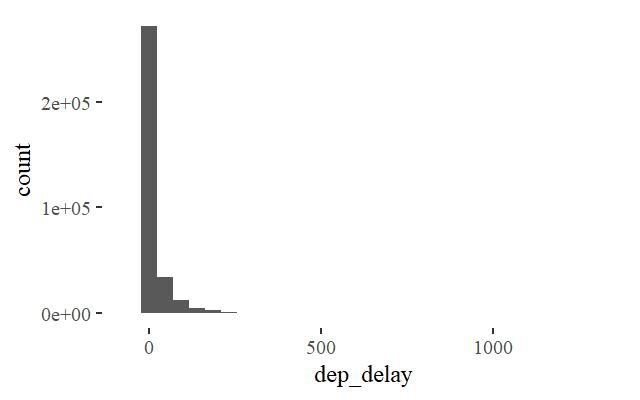
\includegraphics[width=0.75\linewidth,height=0.75\textheight]{flights_analysis_files/figure-latex/unnamed-chunk-1-1}

Above we can see the distances between flight origin and destination.
It's worth mentioning that the longest flights (around 5000 miles) are
all to Hawaii.

\begin{verbatim}
#> `stat_bin()` using `bins = 30`. Pick
#> better value with `binwidth`.
#> `stat_bin()` using `bins = 30`. Pick
#> better value with `binwidth`.
\end{verbatim}

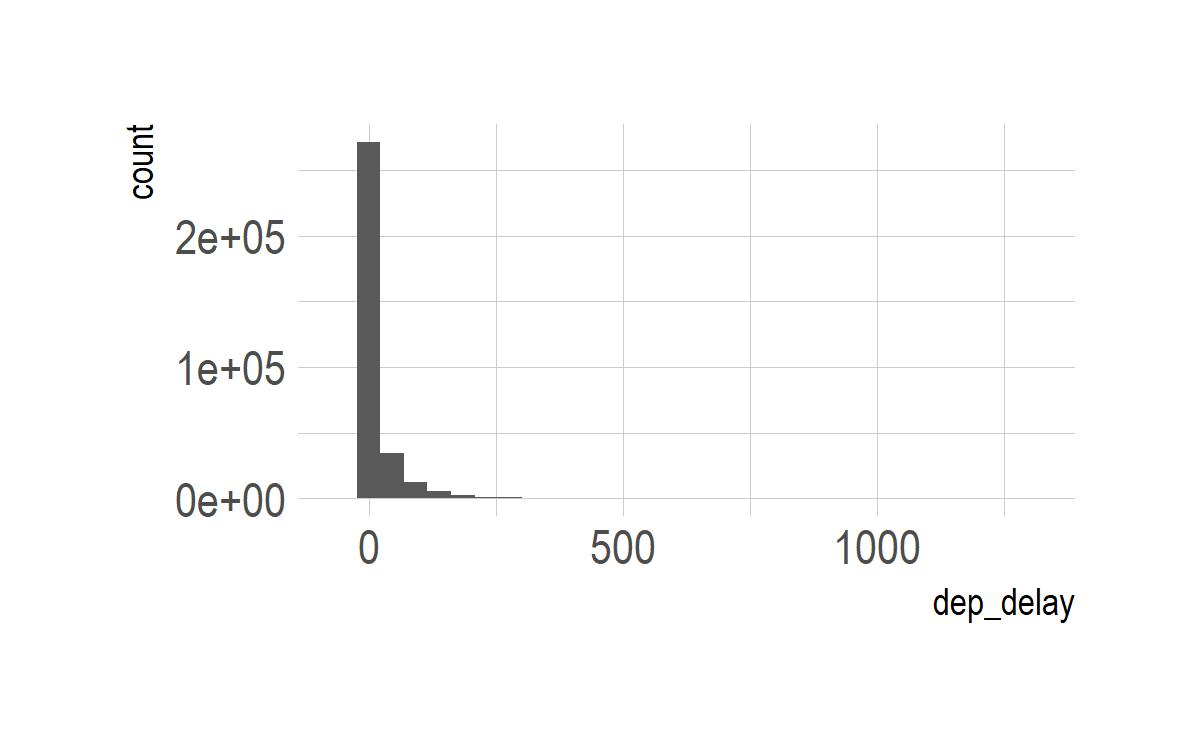
\includegraphics[width=0.75\linewidth,height=0.75\textheight]{flights_analysis_files/figure-latex/unnamed-chunk-2-1}

Above we can see histograms of the actual departure time and the
scheduled departure time.

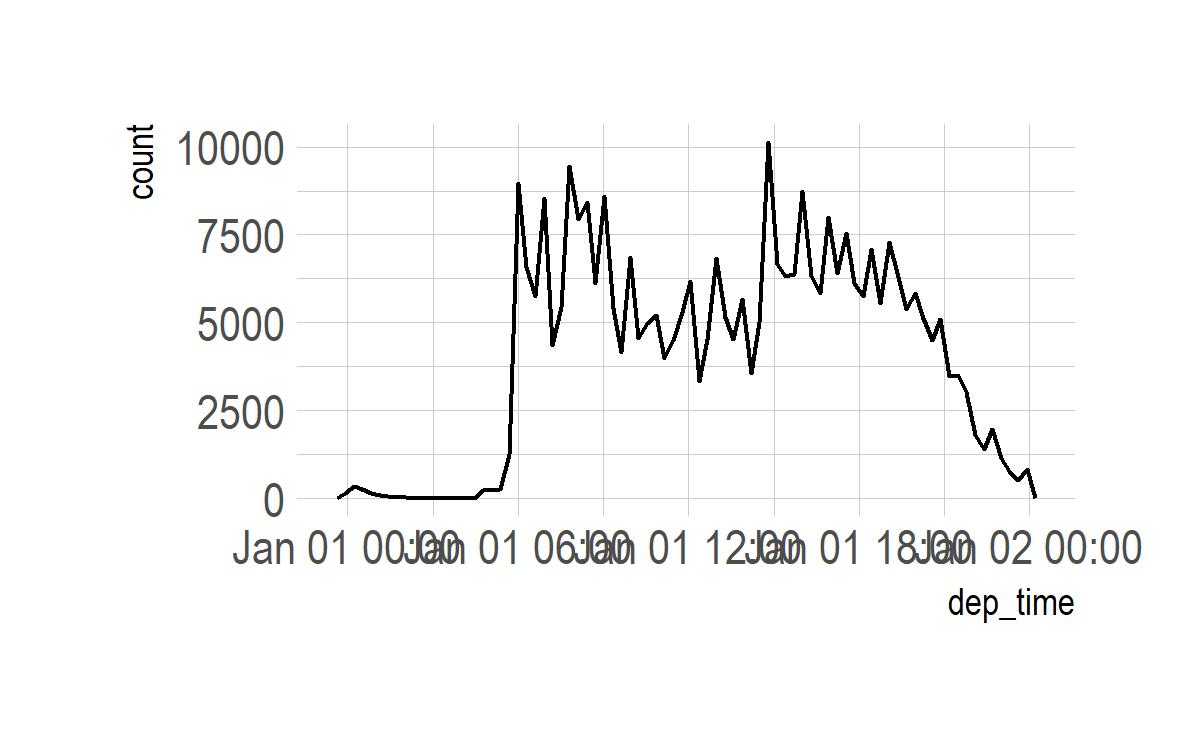
\includegraphics[width=0.75\linewidth,height=0.75\textheight]{flights_analysis_files/figure-latex/unnamed-chunk-3-1}

Most flights appear to leave New York on time, or with slight delays.
The flights in the bottom right corner are flights that left the day
after they were scheduled.

\begin{verbatim}
#> `stat_bin()` using `bins = 30`. Pick
#> better value with `binwidth`.
#> `stat_bin()` using `bins = 30`. Pick
#> better value with `binwidth`.
\end{verbatim}

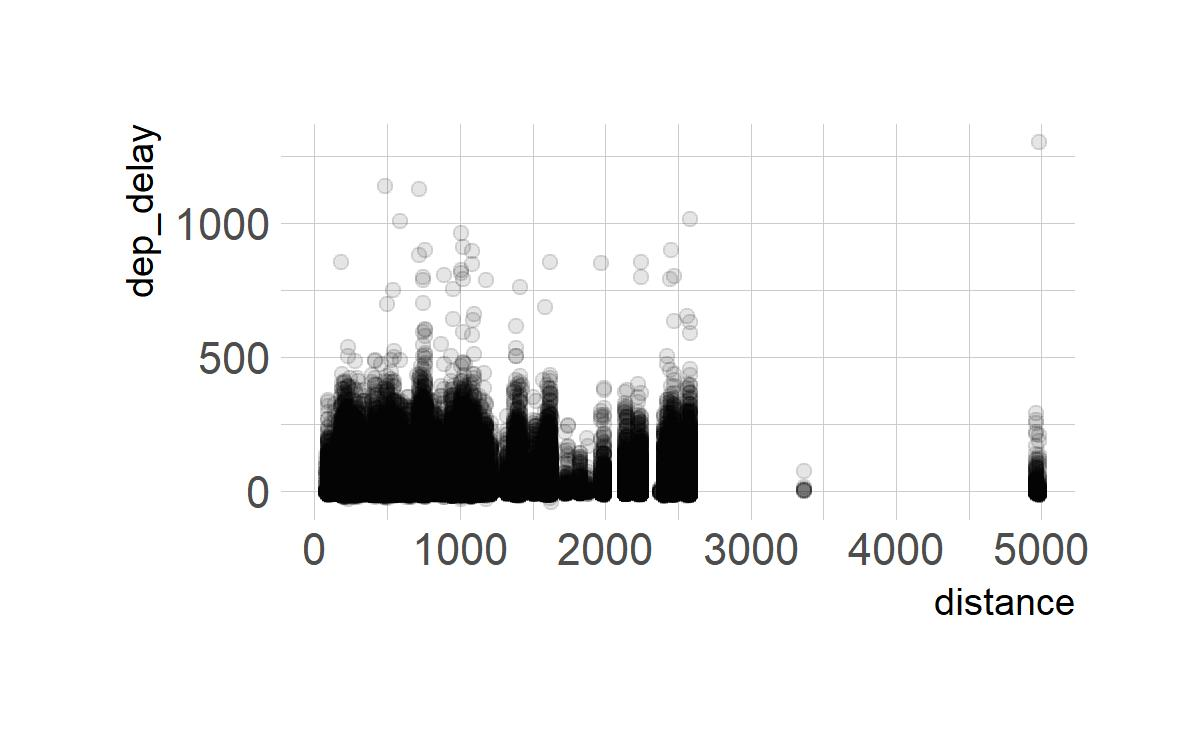
\includegraphics[width=0.75\linewidth,height=0.75\textheight]{flights_analysis_files/figure-latex/unnamed-chunk-4-1}



\end{document}
